%
%
%\citet{DAntona2000} presented the first hints the missing physics, well before the full severity of model deficiencies was understood. They showed that including a rudimentary prescription for the effects of magnetic fields on convection provided better...

\begin{figure}
	\centering
    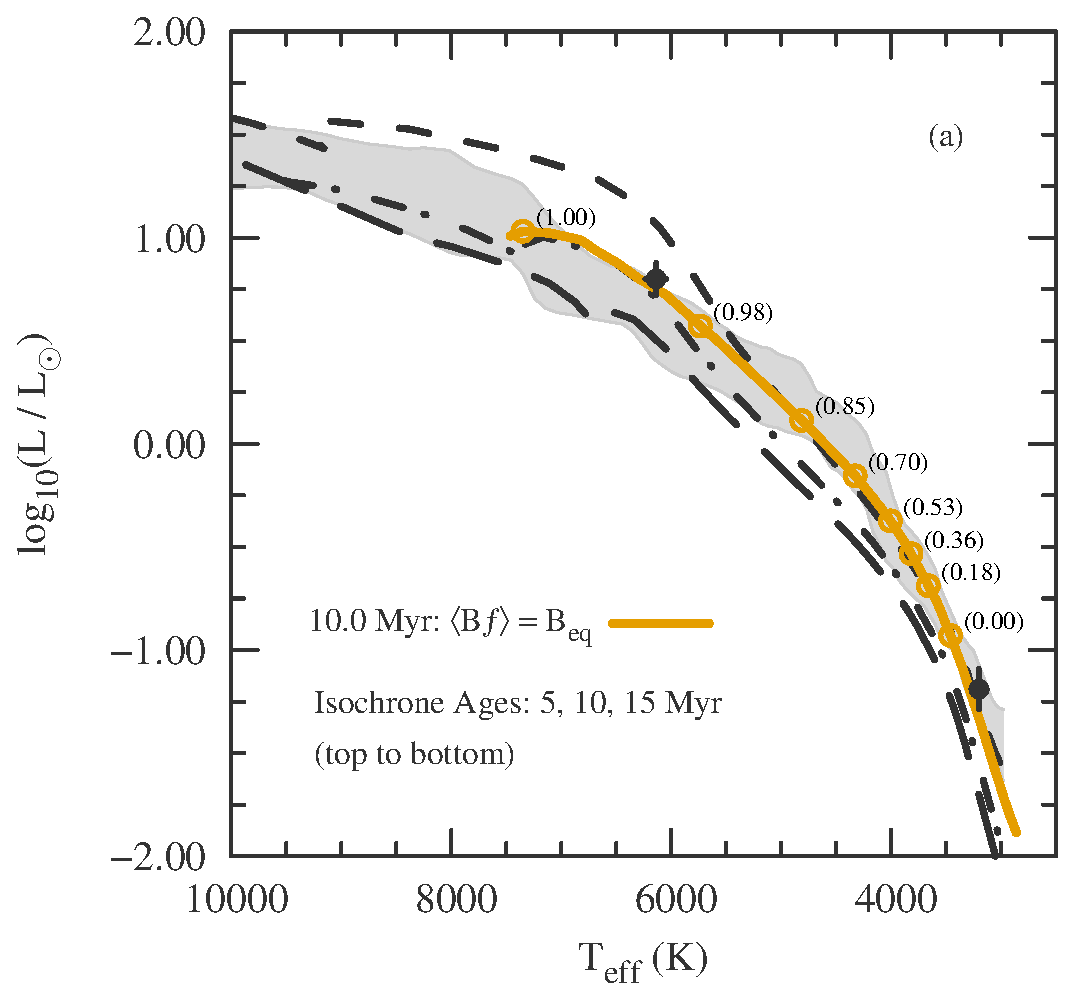
\includegraphics[scale=0.45]{fig/USco_HR_diagram.eps} \hspace{\fill}
    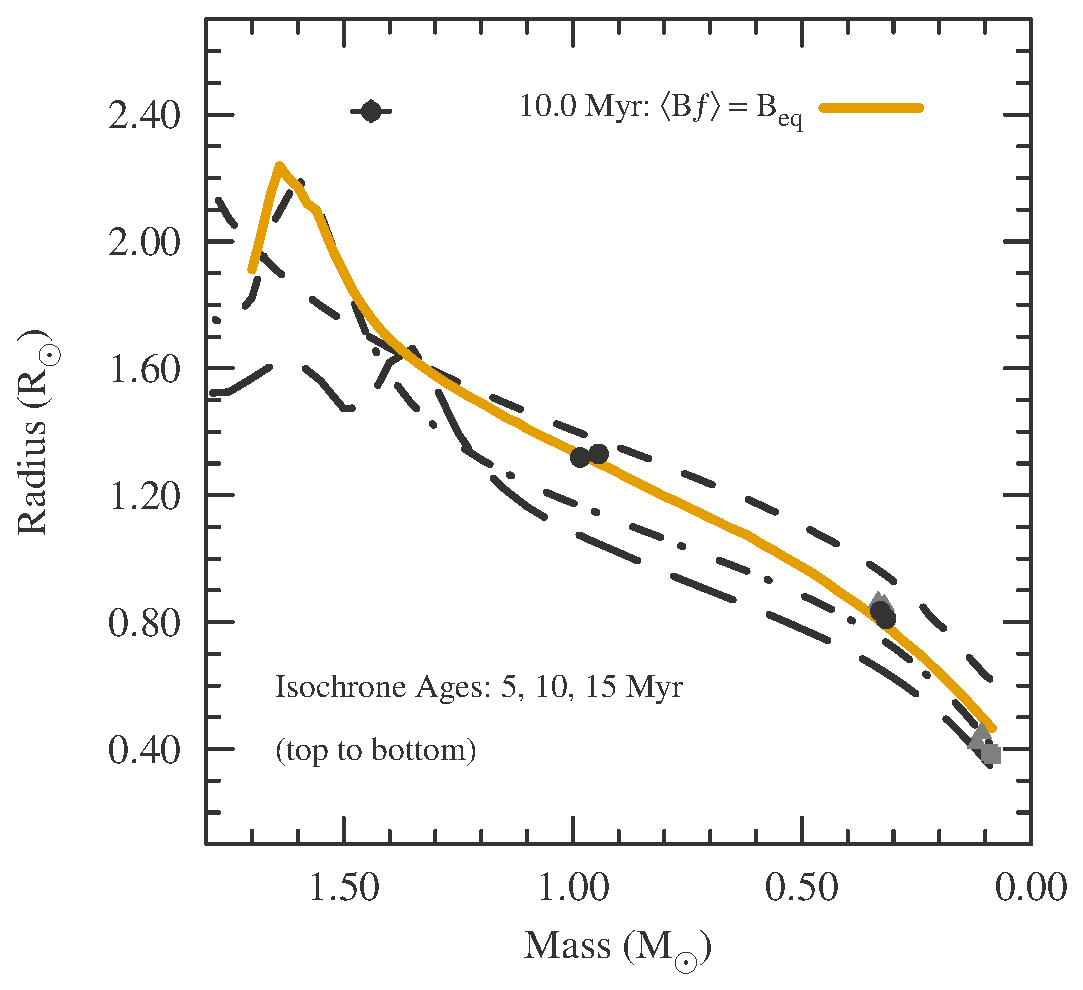
\includegraphics[scale=0.45]{fig/USco_MR_diagram.eps}
    \caption{({\it left}) HR diagram of Upper Scorpius with components of eclipsing binary systems UScoCTIO5 \citep{Kraus2015} and HD 144548 \citep{Alonso2015}
    observed by {\it Kepler}/K2 (black points). A 10 Myr magnetic stellar evolution isochrone is shown by the solid blue line. Note that the 10 Myr magnetic isochrone lies on top of the 5 Myr standard isochrone. ({\it right}) Mass-radius relationship for Upper Scorpius from {\it Kepler}/K2 eclipsing binary systems. {\it Unlike standard models, magnetic stellar evolution models naturally reproduce the slope of the low-mass mass-radius relationship at the same age predicted from the HR diagram.}}
    \label{fig:usco}
    \vspace{-0.2in}
\end{figure}

Recently, our group demonstrated that magnetic fields may provide a viable explanation for observed surface-temperature dependent ages in young clusters and the discordance between HRD and MRD age estimates \citep[see Figure~\ref{fig:usco};][]{Feiden2016}. The hypothesis is that Lorentz forces generated by strong magnetic fields suppresses convective flows in young stars, which acts to cool the stellar surface \citep[e.g.,][]{DAntona2000, MM01, FC12b}. As a result, the contraction of young pre-main-sequence stars is delayed, meaning young stars have cooler temperatures and larger radii at a given age when magnetic inhibition of convection is included in model calculations \citep{MM10, Feiden2016}. The physical mechanism is analogous to formation of sunspots, where strong magnetic fields suppress convection causing the stellar plasma contained within a magnetic region to cool and thus appear darker than its surroundings \citep{Biermann1941, Deinzer1965}. The difference is that sunspots are highly localized phenomena whereas our models consider global-scale magnetic inhibition of convection. 

Previous investigations showed that magnetic inhibition of convection could relieve age disparities between HRD ages and lithium depletion boundary ages \citep{DAntona2000}. For examples, ages inferred from an HRD for cool star members of the $\beta$ Pictoris moving group using standard stellar evolution models indicated the group was 10 Myr old, while the same models provided an age of 20 Myr based on the lithium depletion boundary \citep{Someone2005, Binks2013}. However, by including magnetic inhibition of convection, \citet{MM10} and \citet{Malo2014} showed that the two age estimates could be brought into rough agreement at an age of 25 -- 30 Myr. Shortly thereafter, \citet{Mamajek2014} re-derived an age for high-mass members of the $\beta$ Pictoris moving group and found an age consistent with the magnetic model predictions for the ages of the cool stars. This provided the first hint that magnetism may explain effective-temperature-dependent ages.
%age discrepancies for the 25 Myr old $\beta$ Pictoris moving group \citep{MM10, Malo2014}.

Magnetic models were successful at reconciling the two age estimates, but it was not clear whether the magnetic models were {\it accurate} because HRD and lithium depletion boundary studies are mass agnostic. To know whether magnetic models predict accurate properties for real stars, EBs in well-studied young clusters were needed. Masses and radii measured in EBs provide the most stringent test of stellar models as mass is the primary model input and observationally determined radii are more reliable than $T_{\rm eff}$ and luminosity estimates. Finding EBs in young clusters would also provide an opportunity to confirm the MRD age estimate against an age inferred from an HRD using an independent sample of stars.

A source of EBs in a well-studied young cluster became available when \kepler\ observed the Scorpius-Centaurus OB Association for 80 continuous days. A number of EBs were quickly identified in the Upper Scorpius subgroup, including two EBs for which precise masses and radii were determined \citep{Kraus2015, Alonso2015}. Critically, the two EBs occupied two distinct regions of the MRD thereby defining a preliminary mass-radius relationship (see Figure~\ref{fig:usco}). Comparing the EB mass-radius relation against model predictions, it is clear that standard models predict an incorrect {\it slope} for the mass-radius relationship. Ultimately, models were found to exhibit errors in age by up to 100\% and using the empirical HRD to derive a mass from standard models yields errors in the true mass by up to 50\% \citep{Kraus2015}.

However, when we compare the mass-radius relationship predicted by models that include magnetic inhibition of convection, we find that the model mass-radius relation steepens such that it closely matches the observed relationship at an age of approximately 10 Myr \citep[see Figure~\ref{fig:usco};][]{Feiden2016}. Figure~\ref{fig:usco} also demonstrates that the age predicted by the magnetic models in the MRD provides a reasonable fit to the median HRD sequence. {\bf Magnetic models appear to predict a consistent age in both the HRD and MRD. Furthermore, magnetic models predict an age that is largely independent of effective temperature in the HRD.} What's more, is that the surface magnetic fields strengths used to compute the stellar models were selected {\it a priori} based on arguments that the magnetic field is in thermal equipartition with the surrounding gas, as has been observed among young T-Tauri stars (Johns-Krull et al. 1999), and deep interior magnetic field strengths are of a plausible magnitude (Browning et al. 2016). This means magnetic models are exhibiting some level of predictive power when it comes to reproducing the properties of young stars.

% \citep{JohnsKrull1999}. 
%Results from \citet{Feiden2016} are tantalizing, as they offer a path toward reliable young stellar ages, but important questions remain about the validity and accuracy of these ``magnetic stellar evolution models.'' First, properties of the magnetic field are prescribed in a rather ad-hoc fashion \citep{FC12b, FC13}. Simple functions are used to describe the magnetic field strength as a function of radius deep in a star \citep{FC13}, but the situation in real stars is far more complex and depends intimately on the precise structure and rotational velocity of the star \citep{Browning2008, Brown2010}. Second, the interaction of Lorentz forces on convection depend strongly on the magnetic field topology throughout the star \citep{FC13}. At the moment, models use a free parameter to describe an average magnetic field topology, but the parameter is fixed and not allowed to vary as would be expected for a real magnetic field \citep{FC12b}. Finally, the existing magnetic field framework requires the specification of the surface magnetic field strength \citep{FC12b}. This value is either chosen arbitrarily \citep{FC12b, FC13, FC14, FC14b}, or at best, order of magnitude estimates are used to describe a possible maximum value \citep{Feiden2016}. The latter estimates are consistent with field strengths observed on young T Tauri stars \citep{JohnsKrull1999}, but this provide only indirect support for the model predictions.

%The full effect of these modeling choices are felt when stars are allowed to evolve in time. Properties of the magnetic field are a function of the stellar structure and stellar rotation, which both vary over time. Therefore, magnetic fields are expected to also evolve in time. 

Results from \citet{Feiden2016} are tantalizing, as they offer a path toward reliable young stellar ages, but important questions remain about the validity and accuracy of these ``magnetic stellar evolution models.'' Answers to some of these questions, such as whether model predict the correct mass-radius relationship across the entire MRD, are near at hand thanks to immense efforts to uncover and characterize EBs in young stellar populations with \kepler. However, detailed studies testing new hypotheses, such as magnetic inhibition of convection, are currently hampered by a lack of availability of models that incorporate these new physics (e.g., accretion, magnetic fields, starspots). To make real progress in understanding the observed discrepancies, theoretical models must be available to permit quantitative tests of predictions made by new models. \\


 
%a grid and tools to facilitate adoption of standard and magnetic models is needed to provide a means of testing and magnetic hypothesis.

